\documentclass[10pt,a4paper]{extarticle}
\usepackage[latin1]{inputenc}
\usepackage{amsmath}
\usepackage{microtype}
\usepackage[none]{hyphenat}
\usepackage{verbatim}
\usepackage{amsfonts}
\usepackage{amssymb}
\usepackage{enumitem}
\renewcommand{\familydefault}{\sfdefault}
\usepackage{mathpazo}
\renewcommand{\rmdefault}{put}
\usepackage{enumitem}
\usepackage[dvipsnames,svgnames]{xcolor}
\usepackage{tkz-euclide}
\usetkzobj{all}
\usepackage{graphicx}
\usepackage{tikz} 	
\usepackage{adjustbox}
\usepackage{multicol}
\usepackage{lipsum}
\usepackage[left=0.7cm,right=1cm,top=1cm,bottom=1.5cm]{geometry}
\usepackage{cancel} \usepackage{xcolor}
\usepackage{tcolorbox}
\usetikzlibrary{decorations.pathmorphing,patterns}
\usetikzlibrary{decorations.pathreplacing,calc}
 \newcommand\coret[2][red]{\renewcommand\CancelColor{\color{#1}}\cancel{#2}}
\SetLabelAlign{Center}{\hfil\makebox[1.0em]{#1}\hfil}

%%_------= solusi


% Set this =0 to hide, =1 to show

% Set this =0 to hide, =1 to show
\newtcolorbox{mybox}[1][] { colframe = blue!10, colback = blue!3,boxsep=0pt,left=0.2em, coltitle = blue!20!black, title = \textbf{jawab}, #1, } 

%---------- kunci (jika 1 ) muncul
\def\tampilkunci{1}
\newcommand{\hide}[1]{\ifnum\tampilkunci=1
%
\begin{mybox}
 #1
\end{mybox}
%
\vspace{\baselineskip}\fi}



\newcommand*\cicled[1]{\tikz[baseline=(char.base)]{\node[white, shape=circle, fill=red!80,draw,inner sep=0.5pt](char){#1};}}

\newcommand*\kunci[1]{\ifnum\tampilkunci=1
%
\tikz[baseline=(char.base)]{\node[red, shape=circle,draw,inner sep=0.5pt,xshift=2pt](char){#1};}\stepcounter{enumii}
\fi\ifnum\tampilkunci=0
%
\hspace{3pt}#1\stepcounter{enumii}
%
\fi}

\newcommand*\silang[1]{\tikz[baseline=(char.base)]{
\draw[red,thick](-0.2,-0.20)--(0.2,0.2);
\draw[red,thick](-0.2,0.20)--(0.2,-0.2);
\node[black](char){#1};
}}

\newcommand*\centang[1]{\tikz[baseline=(char.base)]{
\draw[red, very thick](-0.2,0.1)--(-0.1,0)--(0.2,0.3);
\node(char){#1};
}}

\newcommand*\merah[1]{
\textcolor{red}{#1}}
\newcommand*\pilgan[1]{
\begin{enumerate}[label=\Alph*., itemsep=0pt,topsep=0pt,leftmargin=*,align=Center] #1 
\end{enumerate}}
\newcommand*\pernyataan[1]{
\begin{enumerate}[label=(\arabic*), itemsep=0pt,topsep=0pt,leftmargin=*] #1 
\end{enumerate}}

\newcommand{\pilgani}[1]{                            \vspace{-0.3cm}\begin{multicols}{2}
 \begin{enumerate}[label=\Alph*., itemsep=0pt,topsep=0pt,leftmargin=*,align=Center]#1                     \end{enumerate}
 \phantom{ini cuma sapi, wedus, dan ayam}
 \end{multicols}}


\begin{document}


 \textbf{Latihan PAT Cahaya dan Alat Optik} \phantom{ini nama siswa yang aaamengerjakan soal kuis ini }  

\begin{multicols}{3}\raggedcolumns

\begin{enumerate}
\item Seberkas sinar jatuh pada cermin datar PQ dengan sudut datang 60$^o$, kemudian dipantulkan mengenai cermin datar QR. Sudut PQR=135$^o$. Sudut pantul pada cermin QR adalah\\
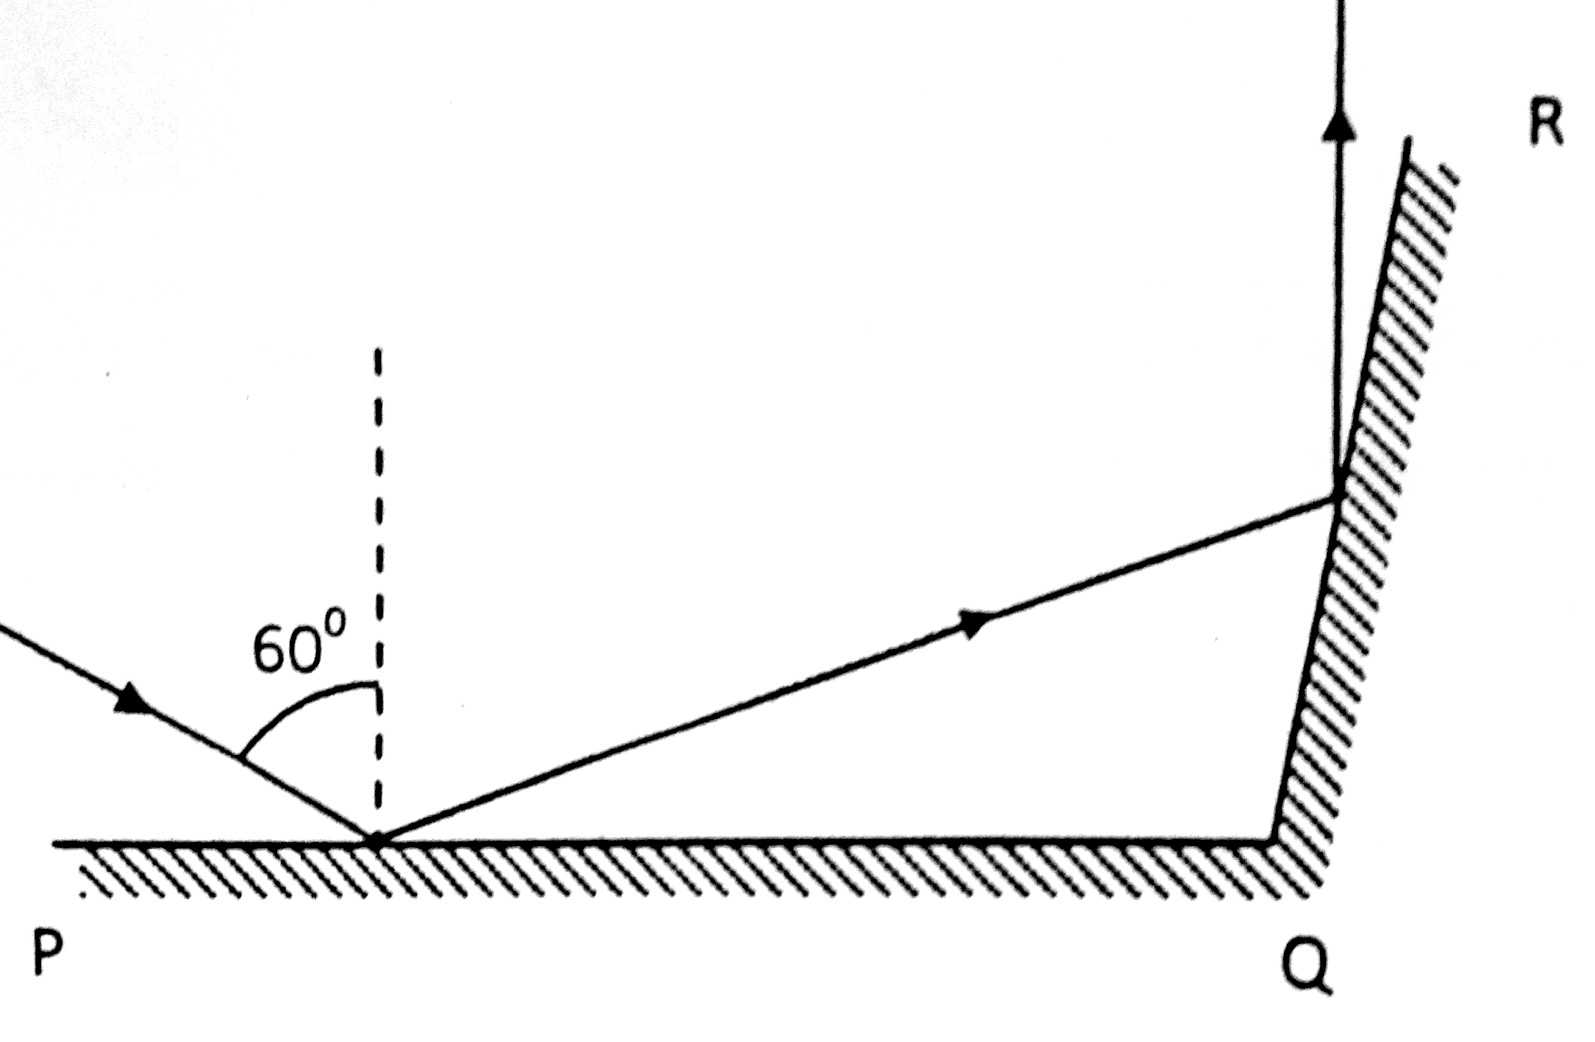
\includegraphics[width=4.5cm]{pic/lab-2}
\pilgani{
   \item 35$^o$
   \item 45$^o$
   \item 55$^o$
   \item 65$^o$
   \item 75$^o$}

\item Dua buah cermin disusun membentuk sudut 40$^o$, maka jumlah bayangna yang terbentuk adalah
\pilgani{
   \item 8 
   \item 9
   \item 10
   \item 11
   \item 12}
\item Bayangan maya yang terbentuk oleh sebuah cermin cekung tiga kali lebih besar dari bendanya. Bila jarak fokus cermin 30 cm, maka jarak benda di depan cermin adalah
\pilgani{
   \item 10 cm
   \item 15 cm
   \item 20 cm
   \item 25 cm
   \item 30 cm}
\vspace{2cm}

\item Sebuah benda diletakkan di depan cermin cembung sejauh 20 cm yang jarak fokusnya 30 cm. Letak dan sifat bayangan yang dibentuk cermin tersebut adalah
\pilgan{
   \item 60 cm depan cermin, maya, tegak
   \item 60 cm blkg cermin, nyata tegak
   \item 60 cm depan cermin, nyata tegak
   \item 12 cm blk cermin, maya, tegak
   \item 12 cm depan cermin, nyata, tegak
}
\vspace{2cm}

\item Benda diletakkan di depan cermin cekung yang jarak fokusnya 15 cm. Jika bayangan yang dihasilkan sama tinginya dengan bendanya maka jarak benda dengan bayangannya adalah
\pilgani{
   \item 0 cm
   \item 15 cm
   \item 30 cm
   \item 45 cm
   \item 60 cm}
   \vspace{2cm}

\item Sebuah benda diletakka 22 cm di depan sebuah lensa dengan jejari 25 cm sehingga diperoleh bayangan di layar yang diletakkan di belakang lensa. Sifat bayangan tersebut adalah
\pilgan{
   \item nyata, terbalik, diperbesar
   \item nyata, terbalik, diperkecil
   \item nyata, tegak, terbesar
   \item maya, tegak, diperbesar
   \item maya, tegak, diperkecil
}
\vspace{2.5cm}

\item Berkas cahaya merambat dari udara dibiaskan ke suatu medium yang mempunyai indeks bias $\frac{1}{2}\sqrt{6}$ dengan arah seperti di gambar. Sudut $\alpha$ pada gambar tersebut adalah\\
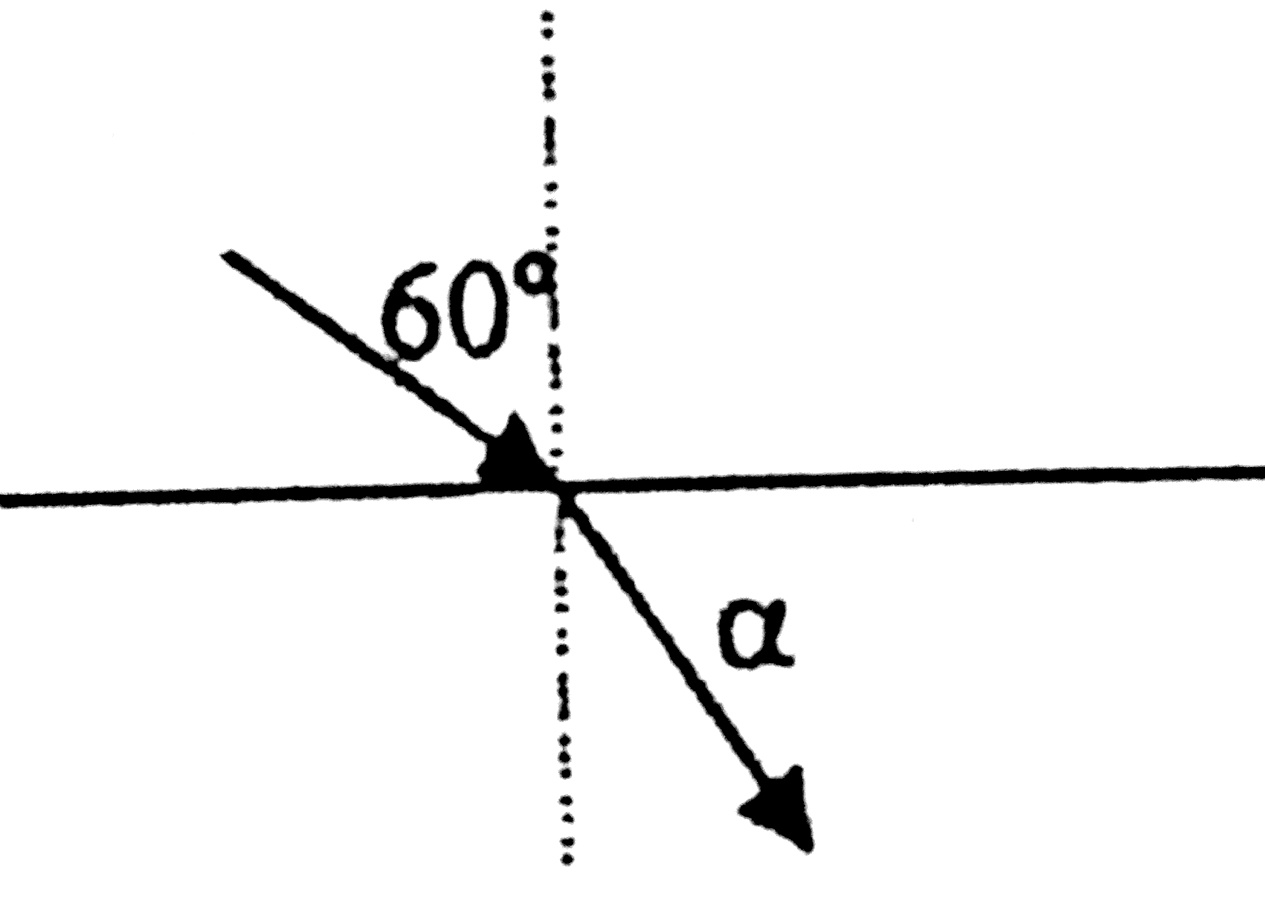
\includegraphics[width=5cm]{pic/lab-3}
\pilgani{
   \item 30$^o$
   \item 37$^o$
   \item 45$^o$
   \item 53$^o$
   \item 60$^o$
}
\vspace{2cm}






\item Titik jauh penglihatan seseorang 100 cm di muka mata. Orang tersebut memerlukan kacamata dengan lensa yang dayanya 
\pilgani{
   \item 0,5
   \item 0,3
   \item -3
   \item -1
   \item 3}

\item Sebuah lensa berjarak fokus 12,5 cm digunakan sebagai lup dengan akomodasi maksimum. Maka perbesaran anguler lup adalah
\pilgani{
   \item 3 
   \item 4 
   \item 5 
   \item 6 
   \item 7}

\item Seseorang tidak dapat melihat benda tak hingga. Setelah itu oleh dokter diberi kacamata -4 dioptri, maka titik jauh mata orang tersebut adalah . . 
\pilgani{
   \item 10 cm
   \item 25 cm
   \item 40 cm
   \item 50 cm
   \item 70 cm
}

\item Titik dekat mata seseorang 400 cm di muka mata.  Agar orang tersebut dapat melihat pada jarak 25 cm, maka perlu kacamata berkekuatan
\pilgani{
   \item 3,75
   \item 3,5
   \item 0,2
   \item -0,2
   \item -0,5 }

\item Titik dekat seseorang adalah 1 m. Maka kuat kacamata yang diperlukan adalah
\pilgani{
   \item 2 D
   \item 3 D
   \item 4 D
   \item 3,5 D
   \item -2 D }

\item Seseorang yang titik dekatnya ada pada jarak 50 cm di depan lensa matanya, hendak membaca buku pada jarak 25 cm. Maka kuat lensa yang harus dipakai adalah
\pilgani{
   \item -2 dioptri
   \item -0,5 dioptri
   \item 2 dioptri
   \item 3 dioptri
   \item 6 dioptri}

\item Sebua lensa berjarak fokus 8 cm digunakan sebagi lup. Jika mata tanpa berakomodasi, maka letak benda tersebut dari lup adalah 
\pilgani{
   \item 2 cm
   \item 3 cm
   \item 4 cm
   \item 6 cm
   \item 8 cm }
\vspace{1.5cm}
\item Sebuah lup dengna kekuatan 20 D digunakan untuk mengamati benda kecil yang berjarak 5 cm dari lup. Perbesaran yang didapatkan adalah
\pilgani{
   \item 12,5 kali
   \item 1,25 kali
   \item 6 kali
   \item 5 kali
   \item 6,25 kali
}
\vspace{1.7cm}
\item Mikroskop memiliki fokus objektif dan okuler 1,5 cm dan 5 cm untuk mengamati preparat pada jarak 2 cm dari lensa objektif. Jika pengamatan dilakukan tanpa akomodasi dengan titik dekat 40 cm, maka perbesaran yang diperoleh adalah
\pilgani{
   \item 24 kali
   \item 32 kali
   \item 30 kali
   \item 20 kali
   \item 36 kali }
   \vspace{2cm}

\item Mikroskop dengan jarak fokus lensa objektif dan lensa okuler berturut - turut 1 cm dan 2,5 cm  digunakan untuk mata normal tanpa akomodasi. Apabila jarak kedua lensa 13,5 cm, jarak preparat terhadap lensa objektif adalah
\pilgani{
   \item 1,3 cm
   \item 1,1 cm
   \item 1,09 cm
   \item 1 cm
   \item 0,9 cm }
\vspace{2cm}

\item Jarak fokus lensa objektif dan okuler 2 cm dan 5 cm, untuk melihat benda 2,5 cm dari lensa objektif. Jika mata normal berakomodasi mksimum, maka perbesaran yang dihasilkan mikroskop adalah
\pilgani{
   \item 20 kali
   \item 24 kali
   \item 25 kali
   \item 50 kali
   \item 54 kali}
\vspace{2cm}

\item Objek pada jarak 1,5 cm dari lensa objektif. Jika fob dan fok 1 cm dan 6 cm, dan titik dekat pengamat 30 cm sedang akomodasi maksimal, maka perbesaran bayangan yang dihasilkan
\pilgani{
   \item 10 kali
   \item 12 kali
   \item 18 kali
   \item 20 kali
   \item 25 kali}
\vspace{2cm}
\item Teropong menghasilkan perbesaran anguler 50 kali untuk mata tak berakomodasi. Jika jarak fokus lensa objektif 250 cm, maka jarak antara lensa objektif dan lensa okuler adalah
\pilgani{
   \item 250 cm
   \item 255 cm
   \item 260 cm
   \item 265 cm
   \item 270 cm
}
\vspace{2cm}

\item Perhatikan gambar berikut.\\ 
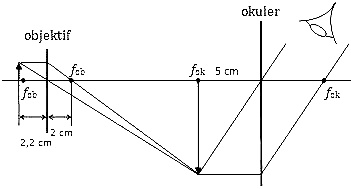
\includegraphics[width=4.5cm]{pic/lab-4}
Maka perbesaran total mikroskop adalah
\pilgani{
   \item 70 kali
   \item 60 kali
   \item 55 kali
   \item 50 kali
   \item 40 kali}
   \vspace{2cm}

\item Sebuah teropong digunakan untuk melihat bintang yang menghasilkan perbesaran anguler 6 kali. Jarak lensa objektif terhadap objektif terhadap okuler 35 cm. Teropong digunakan dengan mata tak berakomodasi, maka jarak fokus okulernya adalah
\pilgani{
   \item 30 cm
   \item 10 cm
   \item 7,5 cm
   \item 5 cm
   \item 3,5 cm
}
\vspace{2cm}

\item Sebuah teropong bintang digunakan tanpa akomodasi oleh seseorang bermata normal. Jika perbesarannya adalah 12 kali  dan fokus lensa objektifnya 72 cm maka panjang teropong tersebut adalah
\pilgani{
   \item 80 cm
   \item 94 cm
   \item 75 cm
   \item 78 cm
   \item 90 cm}

\item Cahaya suatu sumber melalui dua celah sempit yang terpisah 0,5 mm. Jika  jarak antara dua celah semmpint dengan layar 200 cm dan panjang gelombang yang digunakan adalah 600 nm, maka jarak antara garis gelap ke-2 dengan garis terang pusat adalah 
\pilgani{
   \item 9,6 mm
   \item 3,6 mm
   \item 2,8 mm
   \item 2,4 mm
   \item 1,2 mm}
\vspace{2cm}

\item Sebuah celah ganda disinari cahaya 550 nm. Jika layar diletakkan 2 m dari celah dan jarak kedua celah 0,3 mm, maka jarak kedua pita terang yang berdekatan adalah . . .
\pilgani{
   \item 2,5 mm
   \item 3,0 mm
   \item 3,6 mm
   \item 4,5 mm
   \item 5,6 mm
   }
   \vspace{2cm}

  \item Seberkas sinar monokromatis dengan panjang gelombang 5000A melawati celah tunggal menghasilkan pola difraksi orde terang pertama seperti pada gambar. Maka lebar celahnya adalah\\
  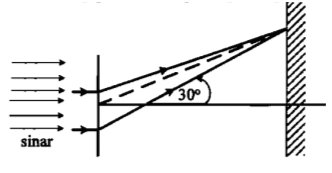
\includegraphics[width=4.5cm]{pic/lab-1}
  \pilgani{
     \item 0,0001 mm
     \item 0,0005 mm
     \item 0,0010 mm
     \item 0,0012 mm
     \item 0,0017 mm}

\vspace{2cm}

\item Sebuah cahaya monokromatik 5000A mengenai kisi 10.000 celah per cm. Garis terang orde pertama teramati pada sudut 30$^o$. Apabila kedua ujung kisi dittup hingga celah yang diamati tinggal 5000, pada sudut tersebut akan diamati . . . .
\pilgan{
   \item garis terang orde pertama
   \item garis terang orde kedua
   \item garis terang orde ketiga
   \item garis gelap orde pertama
   \item garis gelap orde kedua}
\vspace{2cm}

\item Cahaya acak dikenakan pada polarisator vertikal. Cahaya keluaran polarisator dilewatkan pada analisator 60$^o$ terhadap polarisator pertama. Perbandingan intensitas cahaya yang keluar dari analisator terhadap cahaya yang masuk adalah . . 
\pilgani{
   \item 6,25 $\%$ 
   \item 12,5 $\%$
   \item 25 $\%$
   \item 50 $\%$
   \item 100 $\%$
    }

\vspace{2cm}
\item Output polarisator adalah 1/32 intensitas gelombang yang datang. Pada sistem ada 3 polarisator, polarisator pertama sejajar dengan polarisator ke tiga, maka sudut polarisator kedua adalah
\pilgani{
   \item 70
   \item 60
   \item 50
   \item 40
   \item 30}
\vspace{2cm}

\item Radiasi panas matahari yang terkurung dalam atmosfir bumi, serta meningkatnya panas oleh pengikatan CO2 dikenal sebagai . . .  
\pilgan{
\item pemanasan global
\item gas rumah kaca
\item efek rumah kaca
\item polusi suara
\item daya lenting lingkungan}

\item Berikut ini yang \textit{bukan} termasuk akibat dari ``efek rumah kaca'' adalah
\pilgan{
\item berkurangnya areal hutan
\item meningkatnya kematian manusia karena penyakit
\item naiknya suhu bumi
\item turunnya permukaan air laut
\item mencairnya es di daerah kutub}

\item Gas yang timbul dari tempat pembuangan sampah adalah 
\pilgani{
\item SO$_2$
\item O$_3$
\item H$_2$S
\item CO$_2$
\item CH$_4$
}

\item Mekanisme efek rumah kaca yang normal sebenarnya sangat diperlukan bagi kehidupan karena . .
\pilgan{
\item mencegah lubang ozon
\item mengurangi polusi udara
\item menghambat radiasi untuk atmosfer bumi
\item menghangatkan suhu bumi sehingga nyaman untuk ditinggali
\item menyerap gas rumah kaca sehingga tidak terjadi pemanasan berlebihan }

\item Penggunaan CFC pada berbagai produk dibatasi karena
\pilgani{
\item kanker
\item hujan asam
\item keracunan
\item lubang ozon
\item asap kabut}


\item Salah satu dampak pemanasan global adalah
\pilgan{
\item penurunan permukaan laut
\item timbul keracunan CO
\item terjadi gempa
\item rusaknya bahan logam karena korosi
\item timbul penyakit}

\item Penggunaan pendingin (AC, lemari es) berdampak
\pilgan{
\item menipisnya lapisan ozon
\item gangguan pernapasan
\item menipisnya lapisan stratosfer
\item menipisnya atmosfer
\item timbul penyakit kulit}

\item Sumber emisi global yang menghasilkan gas karbon dioksida terbesar adalah
\pilgan{
\item kebakaran hutan
\item pembakaran batu bara
\item penggunaan gas alam
\item kendaraan bermotor
\item kilang minyak}

\item Keuntungan penghijauan antara lain karena tanaman dapat . . .
\pilgan{
\item mengikatkan gas N$_2$
\item menjaga keseimbangan CO$_2$, N$_2$, dan O$_2$
\item mengikat CO$_2$ di udara dan membebaskan O$_2$
\item mengubah CO$_2$ menjadi O$_2$
\item menyerap limbah-limbah industri }


\item Berikut ini yang tergolong gas rumah kaca adalah . . 
\pilgan{
\item CO$_2$, metana, CFC dan oksigen
\item CO$_2$, metana, CFC, dan ozon
\item CO$_2$, metanta, CFC, dan nitrogen
\item metana, CFC, O$_2$, dan uap air
\item metana, CFC, uap air dan helium
}

\item Gas yang dapat menimbulkan hujan asam adalah . . .
\pilgani {
\item SO$_2$
\item O$_3$
\item H$_2$S
\item CO$_2$
\item S$_2$ }

\item Asap kabut dapat menimbulkan kematian karena
\pilgan{
   \item menimbulkan stress
   \item menyebabkan gangguan pernapasan
   \item menimbulkan kelainan pada jantung
   \item mengganggu suplai oksigen
   \item merusak ginjal}

\item Fungsi ozon di lapisan stratosfer adalah
\pilgan{
   \item pelindung bumi dan panas matahari
   \item pelindung bumi dan sinar UV
   \item pelindung bumi dan pengaruh gerhana matahari
   \item pelindung bumi dari pengaruh bintang
   \item semua benar }

\item Meningkatnya kadar karbondioksida di udara dapat menyebabkan 
\pilgani{
   \item rusak lapisan ozon
   \item suhu udara turun
   \item korosi logam
   \item hujan asam
   \item efek rumah kaca}

\item Gas berikut yang dapat mengikat gas ozon sehingga sabuk alam ozon dapat berlubang adalah
\pilgani{
   \item CFC
   \item CH$_4$
   \item H$_2$O
   \item CO$_2$
   \item CO }

\item Ozon dapat dijumpai di atmosfer bumi pada lapisan 
\pilgan{
   \item litosfer dan stratosfer
   \item litosfer dan ionosfer
   \item stratosfer dan ionosfer
   \item stratosfer dan troposfer
   \item troposfer dan ionosfer
}

\item sinar UV matahari hanya sedikit yang sampai ke permukaan bumi karena disaring gas . . .
\pilgani{
   \item O$_3$
   \item CO
   \item NH$_3$
   \item N$_2$
   \item Ar }

\item Gas yang memiliki kemampuan seribu kali lebih efektif dalam mencegah panas keluar dari atmosfer dibanding karbon dioksida dan meyebabkan berlubangnya lapisan ozon adalah . . .
\pilgani{
   \item CO
   \item CH$_4$
   \item CFC
   \item SF$_6$
   \item NO$_2$
}
\item Dampak negatif dari membuang limbah padat sembarangan, \textit{kecuali}
\pilgan{
   \item mengurangi keindahan lingkungan 
   \item menurunkan kualitas tanah
   \item berkembangnya berbagai jenis penyakit
   \item kesuburan tanah meningkat
   \item krisis air bersih}

\item Cara yang dapat dilakuka untuk mencegah meluasnya kerusakan lapisan ozon adalah . . 
\pilgan{
   \item tidak melakukan aktivitas
   \item mengurangi penggunaan bahan ODS
   \item mengadakan penghijauan
   \item mengganti bahan bakar yang ramah lingkungan
   \item tebang pilih kayu hutan
}


\end{enumerate}
\end{multicols}\end{document}






